% ==============================================================================
% Section 4.1: Descriptive Overview
% ==============================================================================
\subsection{Descriptive Overview}
\label{sec:descriptive}

Figure~\ref{fig:timeseries} presents the national monthly time series for each outcome status, disaggregated by sex. A prominent feature of the time series is the sustained increase in registrations across the study period.
National Not Located registrations grew from 275 per month in January 2015 to 1,170 in June 2025, an increase of $+68.2$ cases per year (Newey-West $t = 10.10$, $p < 0.001$).
Located Dead registrations, though smaller in absolute magnitude, nearly tripled from 49 to 144 over the same period ($+8.8$ cases per year, $t = 4.82$, $p < 0.001$).
Located Alive registrations dominate the Total series numerically, contributing 60.0\% of all registrations across the study period, and grew from 790 to 1,788 per month.


\begin{figure}[htbp]
  \centering
  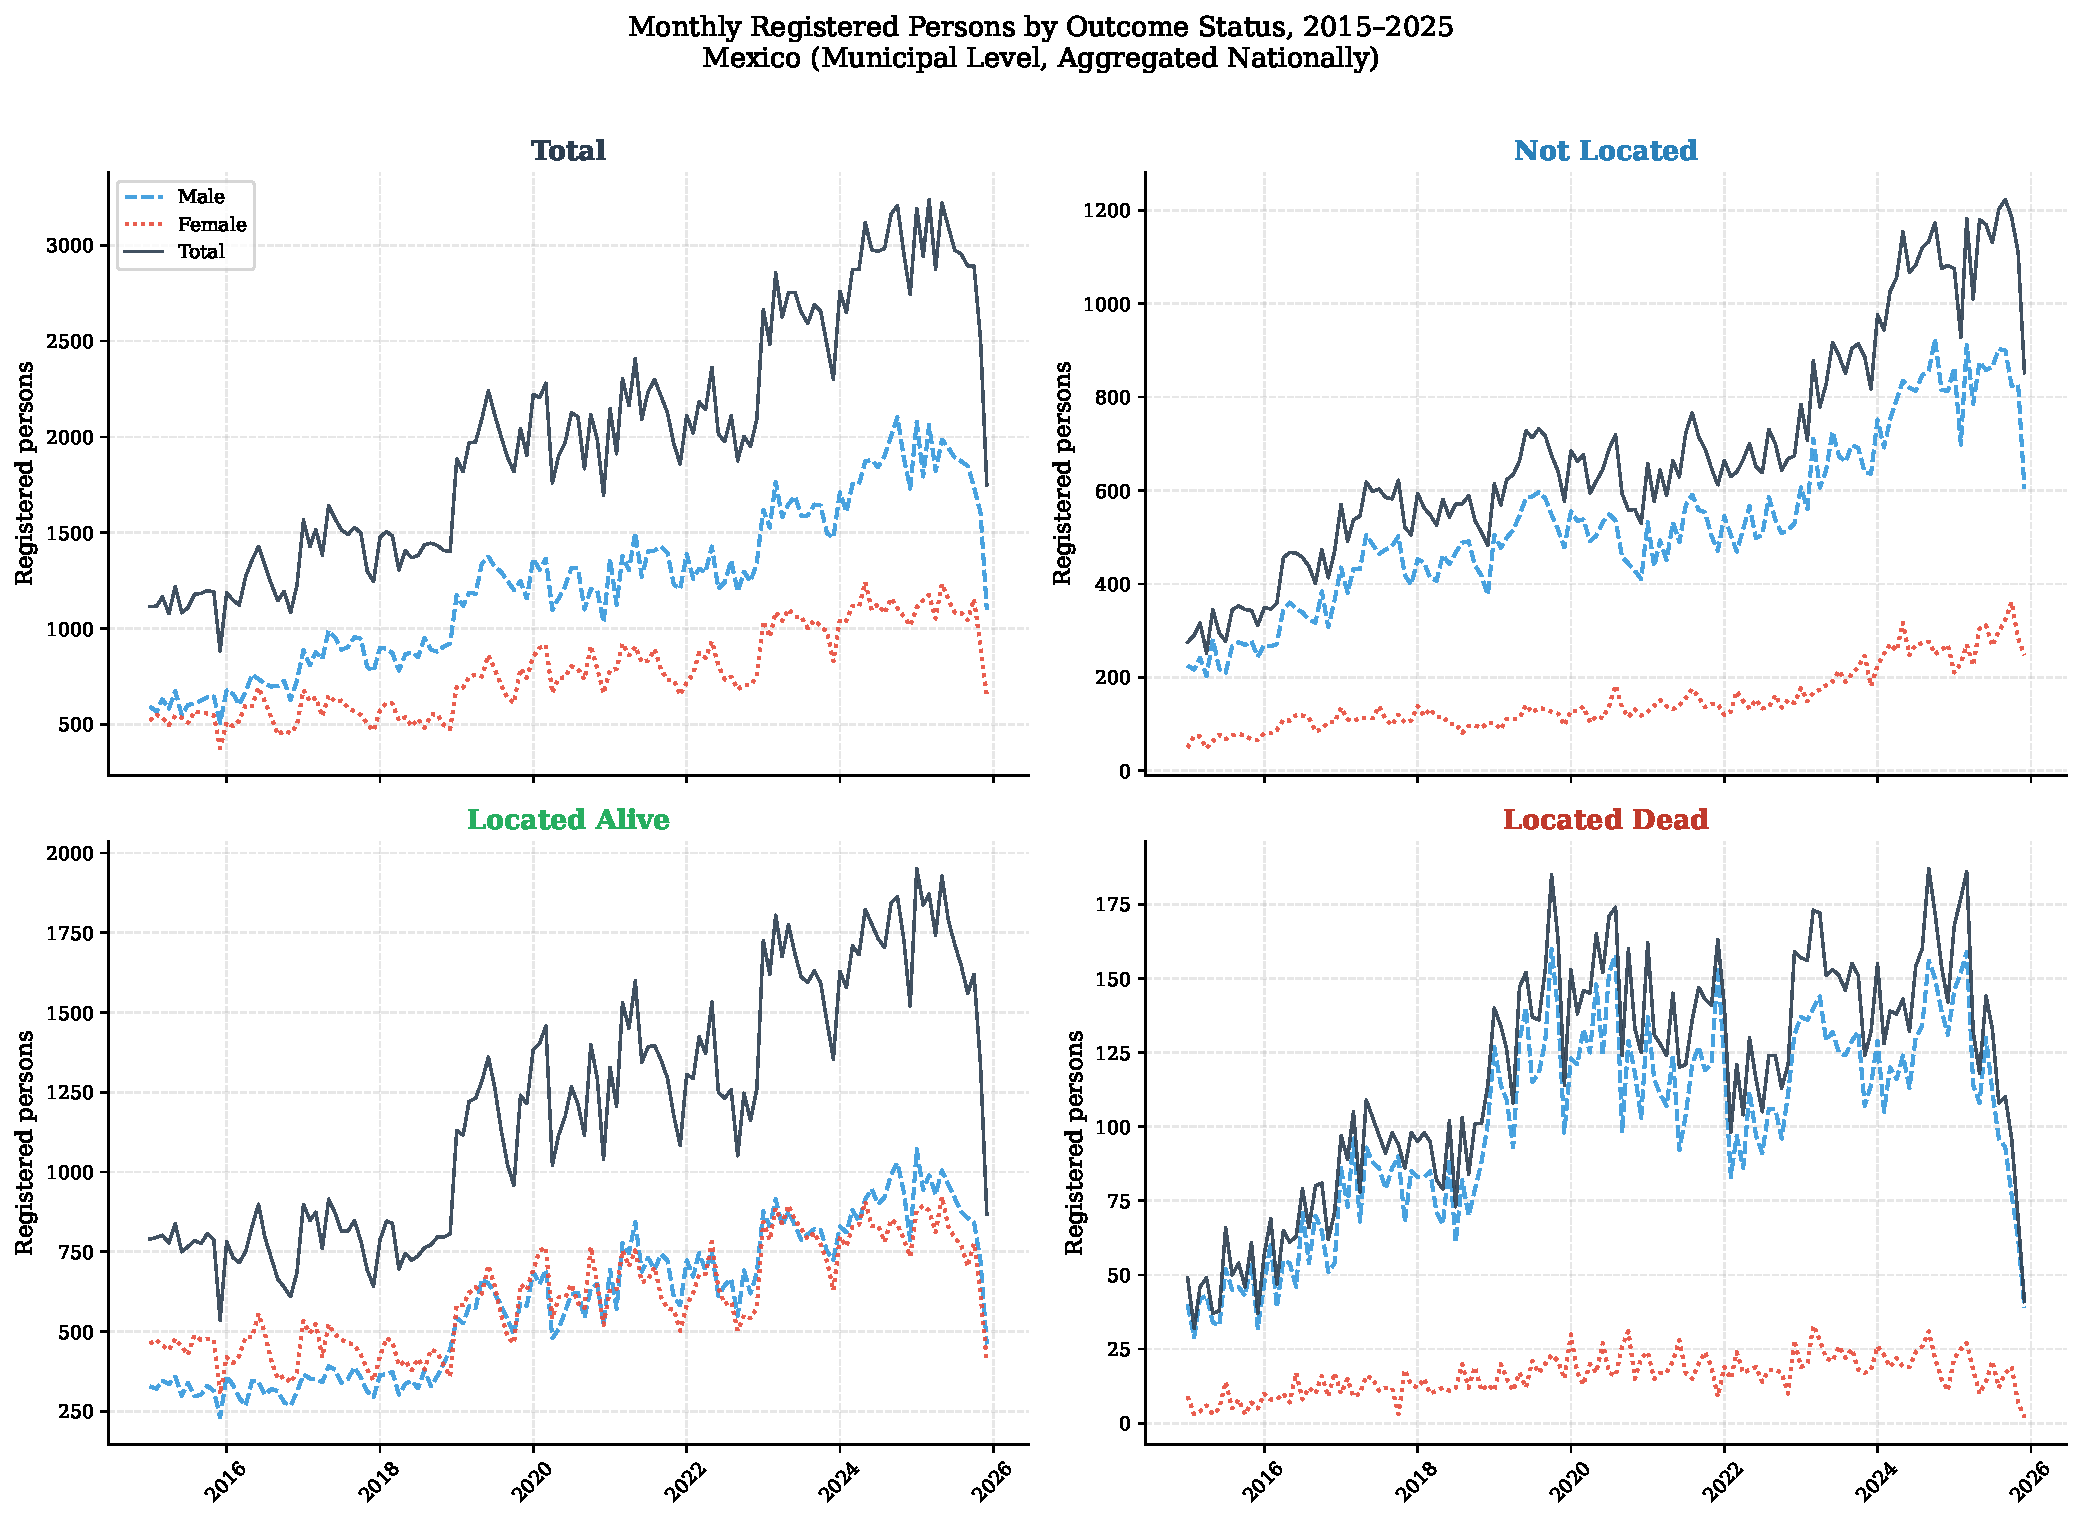
\includegraphics[width=\textwidth]{figures/fig1_time_series_by_status.pdf}
  \caption{Monthly registered persons by outcome status, Mexico, \studyperiod{}.
           Lines show total (solid), male (dashed), and female (dotted)
           case counts aggregated nationally.
           The undefined sex category ($\leq 0.3$\% of registrations) is omitted for clarity.}
  \label{fig:timeseries}
\end{figure}


The sex composition varies markedly across statuses.
Not Located is 77.9\% male, consistent with the established male-dominated profile of disappearance victimization in contexts of organized criminal violence.
Located Dead is even more skewed at 85.9\% male, closely aligned with homicide patterns.
Located Alive, however, approaches near-parity: 49.4\% male and 50.5\% female.
This compositional divergence, where men dominate the population that remains missing while recoveries are gender-balanced, is revisited in Section~\ref{sec:sex}.

Monthly case counts are overwhelmingly zero at the municipality level.
In \referencemonth{}, 77.0\% of municipalities recorded zero Total cases, rising to 85.7\% for Not Located, 84.2\% for Located Alive, and 96.3\% for Located Dead.
All four statuses exhibit extreme right-skew (skewness 11.0 to 21.4): a small number of municipalities contribute disproportionately large counts, a pattern quantified in Section~\ref{sec:concentration_results}.


